% Setup - do not change
\documentclass[11pt]{article}
\usepackage[top=0.9in, left=0.9in, bottom=0.9in, right=0.9in]{geometry} 
\usepackage{parskip}

\usepackage[english]{babel}
\usepackage[utf8]{inputenc}
\usepackage{amsmath,amsthm,amssymb,graphicx,pdfpages,lipsum,hyperref}
\usepackage[none]{hyphenat}
\usepackage{csquotes}
\usepackage{tabularx}
\usepackage{booktabs}
\usepackage{subcaption}

\setlength\parindent{0pt}
%%%%%%%%%%%%%%%%%%%%%%%%%%%%%%%%%%%%%%%%%%%%%%%%%%%%%%%%%%%%%%%%%%%
% add other packages here if required

%% Bibliography are specified in this file. You can also choose inline bib style if you want to. But make sure your citation style is consistent (and proper)
% For more details on citation: https://library.unimelb.edu.au/recite
\usepackage[sorting = none]{biblatex}
\addbibresource{references.bib}

%%%%%%%%%%%%%%%%%%%%%%%%%%%%%%%%%%%%%%%%%%%%%%%%%%%%%%%%%%%%%%%%%%% the '%' symbol denotes comments

% Begin document creation
% DELETE THE \lipsum PLACEHOLDERS WHEN YOU BEGIN
\title{\textbf{Predicting Taxi Trip Duration in NYC}}
\author{
Zihan Yin \\
Student ID: 1149307 \\
\href{https://github.com/MAST30034-Applied-Data-Science/mast30034-project-1-ZihanYin12138}{Github repo with commit}
}

\begin{document}
\maketitle

\section{Introduction}
With the advent of the technology age, mobile phones and the internet have become integral to our daily lives. Nowadays, when people need to get around, they may be more inclined to summon a taxi directly through a mobile app rather than the traditional hand waving on the street. Yellow Taxi, New York's most iconic and traditional taxi service company, is facing a turning point of the times. If they fail to adapt and adopt new tech trends on time, they are likely to be replaced by emerging online taxi platforms.

Considering this challenge, it is assumed that Yellow Taxi has decided to transition online and plans to develop a mobile app to serve its customers better. To this end, our report examines Yellow Taxi's trip duration to provide accurate trip duration forecasts for the company's app. Our report is aimed at the following people interested in trip length: passengers, taxi drivers, Yellow Taxi's management team, and relevant agencies responsible for traffic and road management in New York (e.g., the New York City Transit Authority).

\subsection{TLC Data}
This study uses Yellow Taxi trip data provided by New York City, available at NYC TLC Trip Record Data\cite{TLC_data}. Each record describes a trip in detail, including various features such as boarding location, boarding time, and trip distance.

We analyzed records from January 2019 to June 2019 specifically for data selection. There were two primary considerations for the selection of this period:

\begin{enumerate}
    \item \textbf{COVID-19 impact}: Considering trip duration could be affected by the subsequent COVID-19 outbreak, we wanted to avoid this potential bias by selecting data before the outbreak.
    \item \textbf{Rise of online taxi market}: We see the first half of 2019 as a period of rapid growth for online taxi market, which could be a critical turning point for Yellow Taxi if they plan to expand online.
\end{enumerate}

\subsection{External Data}
In addition to Yellow Taxi's trip data, we used an external dataset from Visual Crossing's Weather Data Services covering January 2019 to July 2019 weather information for New York City\cite{external_data}. We chose one more month of data than the TLC data to facilitate the testing of the model part.

Each row in this weather dataset describes in detail the weather conditions in New York City on a particular day, including essential features such as actual temperature, body temperature, humidity, etc. The main reason we chose to introduce weather as an external dataset is that, intuitively, weather conditions significantly impact trip duration.

Below is a brief overview of the raw TLC data and external weather data.

\begin{table}[h]
\centering
\begin{tabular}{|c|c|c|}
\hline
\textbf{Datasets} & \textbf{num of instances} & \textbf{num of features} \\ 
\hline
TLC Data & 44658561 & 19 \\ 
\hline
External Data & 212 & 33 \\ 
\hline
\end{tabular}
\vspace{-5pt}
\caption{Dataset Shapes} 
\label{tab:dataset_description} %
\end{table}

\section{Preprocessing}
\subsection{Feature Engineering}
%\subsubsection{For TLC Data}
We derived a new set of features from the original TLC data to explore the factors associated with \textit{trip duration}. Although these features were not present in the original data, we believe they strongly correlate with trip duration.

\begin{itemize}
    \item \textbf{Temporal features}: We extracted a feature named \textit{date}, which includes only month and day information for subsequent merging with external data.
    
    \item \textbf{Continuous features}: There are 2 continuous features, \textit{trip duration} (in s) and \textit{average speed} (in miles/h).
    
    \item \textbf{Discrete features}: We generated the following discrete features:
    \begin{itemize}
        \item \textit{if weekend}: Indicates whether it is a weekend.
        \item \textit{if morning peak} and \textit{if evening peak}: Indicate whether it is the morning and evening peak hour, respectively. These 2 features are further used to generate the \textit{if peak hour} and are excluded in the subsequent steps.
        \item \textit{if overnight}: Indicates whether it is late night.
        \item \textit{if airport}: Indicates whether it is to or from the airport.
    \end{itemize}
    These discrete features are binary, where 1 means "yes" and 0 means "no".
\end{itemize}
With the above feature engineering, the number of features in the TLC data was increased from 19 to 28, while the number of instances remained the same.

%\subsubsection{For External Data}
For the external dataset of weather, it covers a wide range of different features. We noticed the existence of a feature called \textit{conditions}, which provided a large amount of helpful information and integrated some information from other features. From this, we extracted vital information and created several new features. Firstly, we constructed a temporal feature \textit{date}, extracting only the month and day from the original temporal feature to facilitate subsequent integration with the TLC data. Second, we created five discrete features based on the conditions feature: \textit{if rain}, \textit{if snow}, \textit{if overcast}, \textit{if cloudy}, and \textit{if clear}. Similar to the newly created discrete features in the TLC data, these five features take the value of either 0 or 1, where 1 represents "yes" and 0 represents "no". After the above feature engineering, the number of features for the external data increased from 33 to 39, while the number of instances remained the same.

\subsection{Remove Invalid Instances and Useless Features}
%\subsubsection{For TLC Data}
Based on Yellow Taxi's data dictionary\cite{TLC_data_dictionary}, we found many instances in TLC data that did not match business rules or were considered invalid. For the accuracy of data, we cleaned or adjusted these instances:

\begin{itemize}
    \item In order to ensure the standardization of \textit{payment\_type}, we kept the values (1 and 2) corresponding to the payment type "credit card" and "cash". 
    \item Removed \textit{RatecodeID} values that were not in the range of 1 to 6.
    \item Only \textit{store\_and\_fwd\_flag} with values 'Y' and 'N' are retained.
    \item Deleted \textit{fare\_amount}, \textit{tip\_amount}, \textit{total\_amount}, \textit{number of passengers}, \textit{trip\_distance}, \textit{extra\_fee}, \textit{trip\_duration}, and \textit{average\_speed} that are less than or equal to 0.
    \item Since \textit{mta\_tax} and \textit{improvement\_surcharge} are fixed fees, we retained only the values of 0.5 and 0.3, corresponding to these two features, respectively.
    \item In \textit{congestion\_fee}, lots of instances are null, which we assume the congestion fee was not incurred during the trip, or was not recorded for some reason, so we replace these null values with 0.
\end{itemize}

After the above processing, the number of instances of TLC data decreased from 44658561 to 26163008.

After the initial data cleaning, we further removed 15 features from the TLC data:

\begin{enumerate}
    \item We removed 9 features that were not related or causally related to travel time, which cannot be used for prediction. The main ones were different types of fees: \textit{VendorID}, \textit{RatecodeID}, \textit{store\_and\_fwd\_flag}, \textit{payment\_type}, \textit{fare\_amount}, \textit{mta\_tax}, \textit{improvement\_surcharge}, \textit{tip\_amount}, and \textit{total\_amount}.
    
    \item 4 features, from which essential information was previously extracted to create new features, were discarded: \textit{pickup\_time}, \textit{dropoff\_time}, \textit{if\_morning\_peak}, and \textit{if\_evening\_peak}.
    
    \item Two features, deemed redundant due to overlaps with others, were also eliminated: \textit{airport\_fee} and \textit{extra\_fee} were found to coincide with \textit{if\_airport}. Moreover, all entries under \textit{airport\_fee} were null, prompting its removal.
\end{enumerate}

2 features that were considered redundant due to overlap with other features were also removed: \textit{airport\_fee} and \textit{extra\_fee} were found to overlap with \textit{if\_airport} and \textit{toll\_fee}. In addition, all instances under \textit{airport\_fee} were null, so they were removed.

After feature removing, the number of features in the TLC data is reduced from 28 to 13.

%\subsubsection{For External Data}
After examining the external data, we found that the dataset had high quality with no invalid instances. Therefore, we directly remove the features that are not useful or have had information extracted from them. In the end, we saved 9 features:

\begin{itemize}
    \item The 6 features generated during our feature engineering step above.
    \item 3 continuous features: \textit{temperature} (temperature body feels like), \textit{uv\_index} (ultraviolet ray intensity), \textit{visibility} (visual clarity).
\end{itemize}


\subsection{Remove Outliers}

There were 5 features in TLC data that we thought may have outliers: \textit{trip\_distance}, \textit{trip\_duration}, \textit{average\_speed}, \textit{congestion\_fee}, and \textit{toll\_fee}. By plotting the box plot, we found that \textit{congestion\_fee} did not have outliers (Figure 1).

\begin{figure}[h]
  \centering
  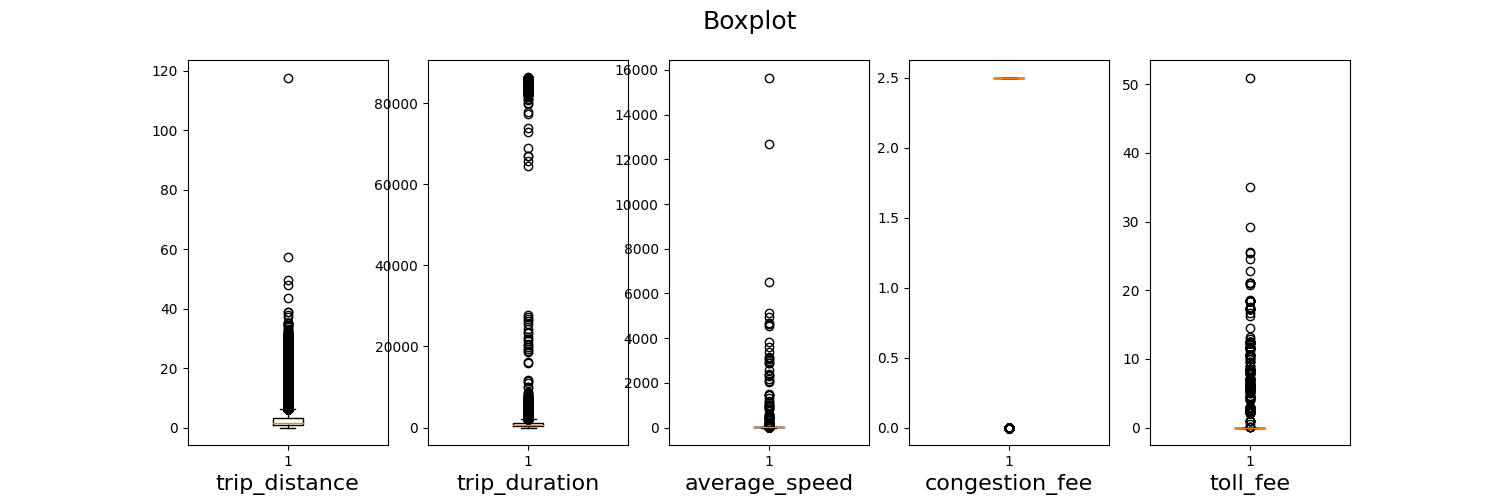
\includegraphics[width=1\textwidth]{boxplot_for_detecting_outlier_1.png}
  \caption{Boxplot for Detecting Outliers (Sample size $=$ 0.01)}
  \label{fig:my_label}
\end{figure}

For the other 4 features, we used the IQR method to remove outliers.

\begin{figure}[h]
  \centering
  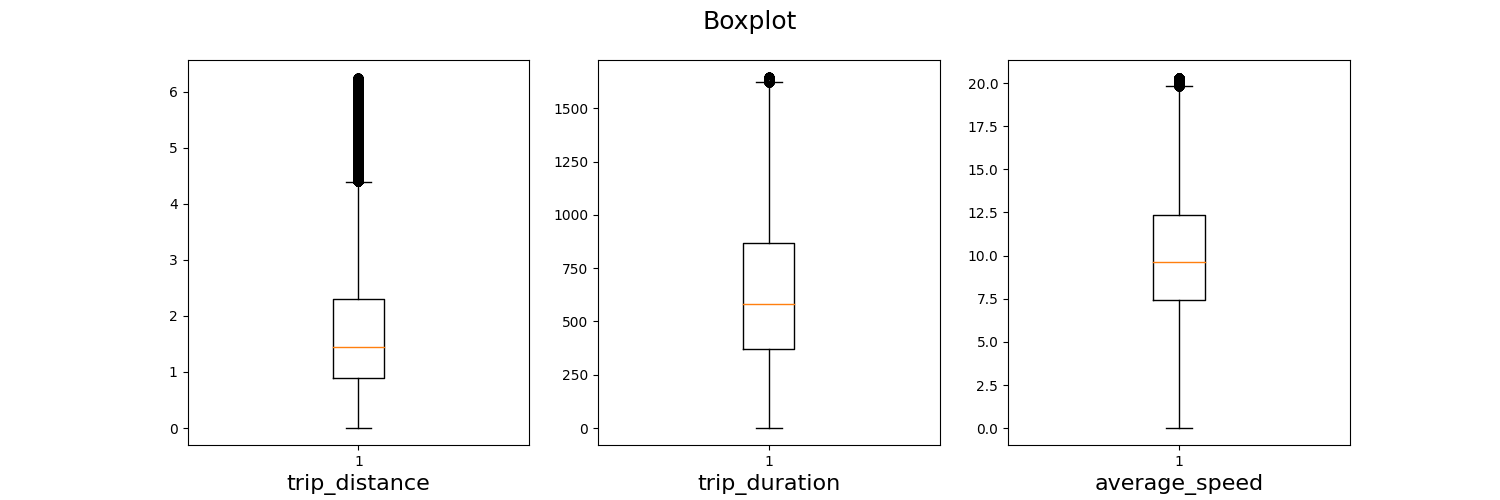
\includegraphics[width=1\textwidth]{boxplot_for_detecting_outlier_2.png}
  \caption{Boxplot After Removing Outliers (Sample size $=$ 0.01)}
  \label{fig:my_label}
\end{figure}

In fact, after applying this method to \textit{toll\_fee}, we found that all values were considered as outliers and removed. Considering that this method may be too strict for \textit{toll\_fee} feature, we decide not to remove its outliers. After the above processing, we left-joined curated TLC data with external data based on \textit{date} feature. The merged data had 22,015,147 instances and 21 features.

\section{Geospatial Visualisation}

We initially hypothesised that \textit{trip duration} has a strong correlation with \textit{location id}. To verify this, we decided to use geospatial plots to check whether different locations have a significant effect on \textit{trip duration}. To do this, we created aggregated data for \textit{up\_location\_id} and \textit{off\_location\_id} using the merged data and calculated the \textit{average trip duration} corresponding to each location. Afterwards, we merged these 2 sets of aggregated data with taxi zones data based on \textit{location id} separately. Based on these two aggregated data, we plotted 2 choropleth maps: Average Trip Duration for Pickup Location (Figure 3) and Average Trip Duration for Dropoff Location (Figure 4). Finally, we marked the top 10 locations with the longest \textit{average trip duration} on these 2 plots.

\begin{figure}[h!]
  \centering
  \begin{minipage}[b]{0.45\textwidth}
    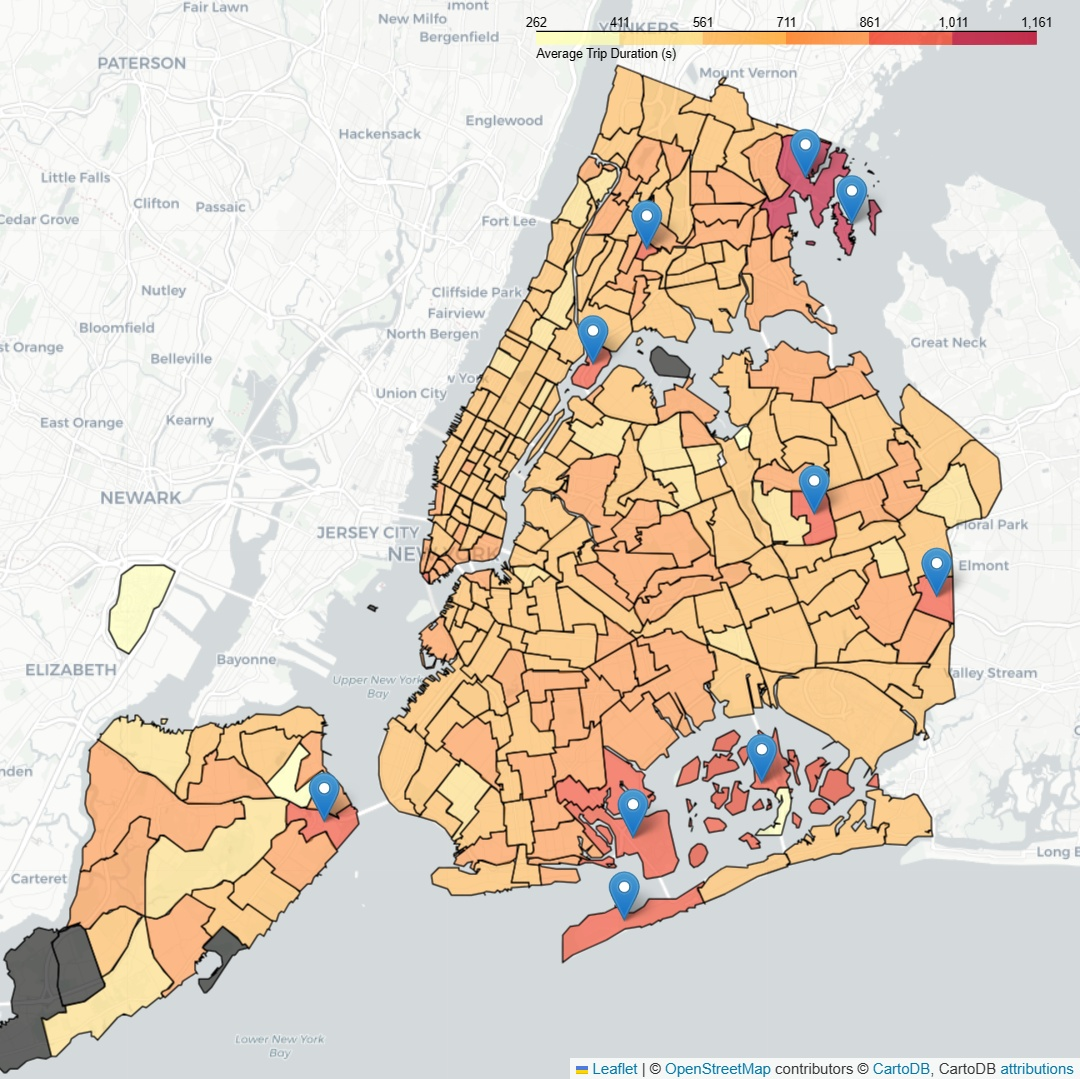
\includegraphics[width=\textwidth]{top10_avg_trip_duration_for_pickup_location.jpg}
    \caption{Top 10 Average Trip Duration for Pickup Location}
    \label{fig:image1}
  \end{minipage}
  \hfill
  \begin{minipage}[b]{0.45\textwidth}
    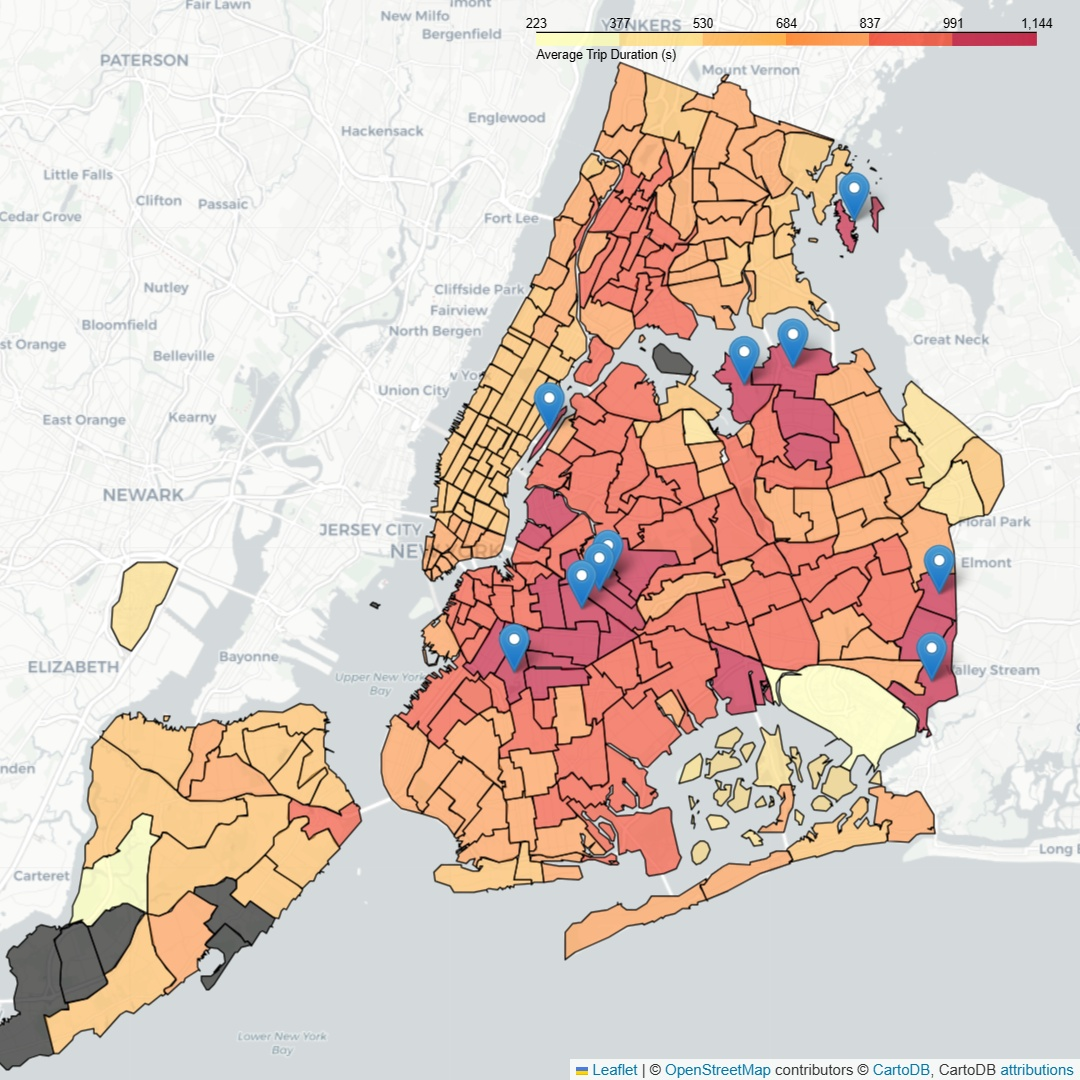
\includegraphics[width=\textwidth]{top10_avg_trip_duration_for_dropoff_location.jpg}
    \caption{Top 10 Average Trip Duration for Dropoff Location}
    \label{fig:image2}
  \end{minipage}
\end{figure}

After observing the geospatial maps, we noted an interesting phenomenon in Figure 3: 7 of the top 10 locations with the longest average trip duration are seaward or island areas: Fort Wadsworth, Floyd Bennett Field,Riis Beach, Jamaica Bay, Randalls Island, Pelham Bay Park, and City Island. Similarly, in the map based on \textit{dropoff\_location\_id}, 4 of the locations, Roosevelt Island, College Point, Whitestone, and City Island, are also by the sea or islands (Figure 4). This observation is discussed in depth in \hyperref[sec:discussion]{Discussion} section. In general, these 2 maps demonstrate that there is a significant difference in the average trip duration between different locations, which further demonstrates the strong relationship between \textit{trip duration} and \textit{location id}. In further work, we can also consider \textit{pickup\_location\_id} and \textit{dropoff\_location\_id} separately and investigate whether they have an interaction effect on \textit{trip duration}.

\section{Plotting and Analysis}

We first plotted the distribution of \textit{trip\_duration}. After observation, we found the distribution of the feature showed a positive skewness. To get a shape close to the normal distribution, we performed a log transformation on 
\textit{trip\_duration}. However, the transformed distribution showed a left skew.

\begin{figure}[h!]
  \centering
  \begin{minipage}[b]{0.45\textwidth}
    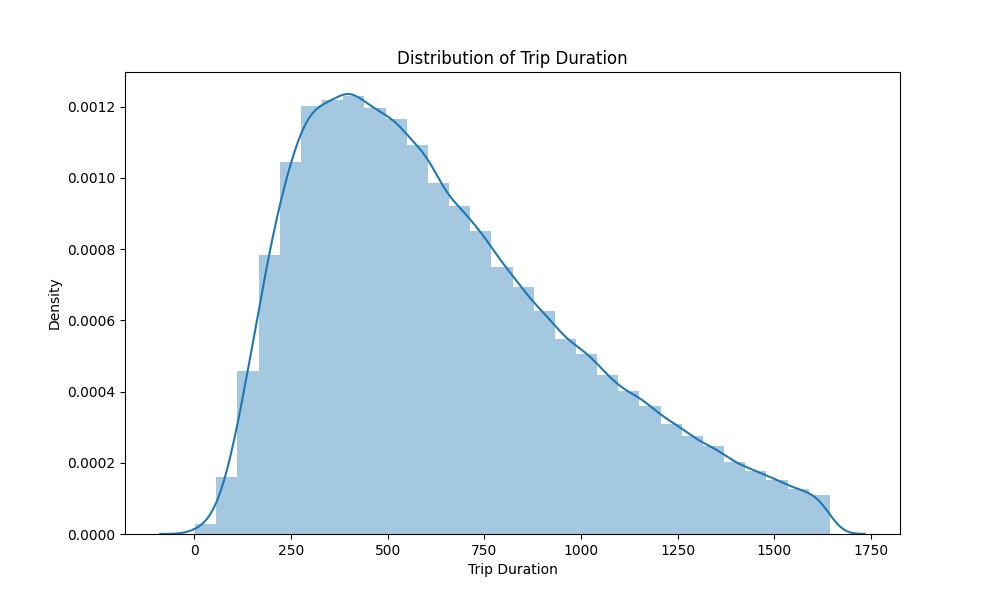
\includegraphics[width=\textwidth]{distribution_of_trip_duration.png}
    \caption{Distribution of Trip Duration (sample size $=$ 0.01)}
    %\vspace{1.3em}
    \label{fig:image1}
  \end{minipage}
  \hfill
  \begin{minipage}[b]{0.45\textwidth}
    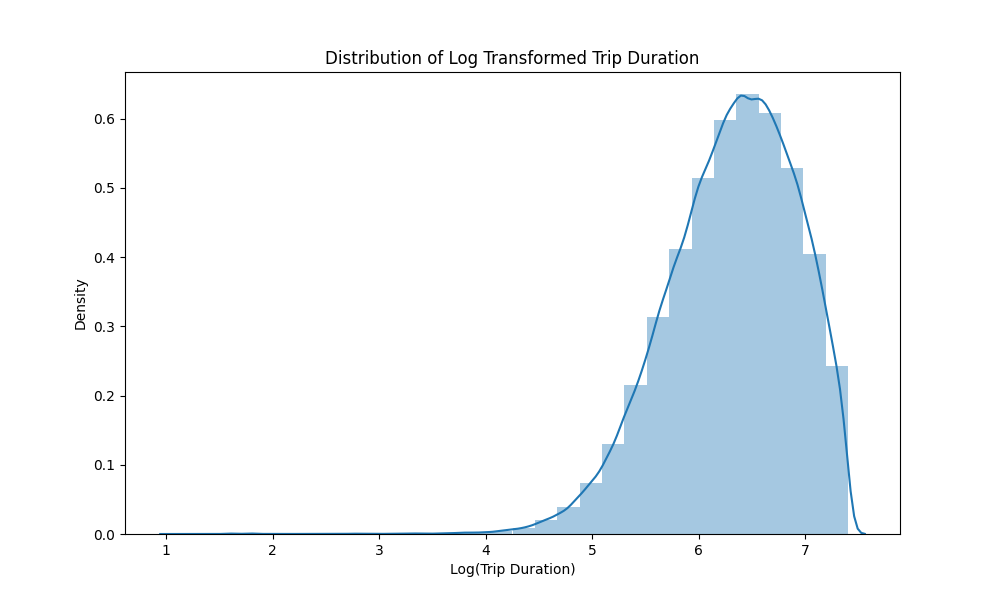
\includegraphics[width=\textwidth]{distribution_of_log_transformed_trip_duration.png}
    \caption{Distribution of Log Transformed Trip Duration (sample size $=$ 0.01)}
    \label{fig:image2}
  \end{minipage}
\end{figure}

To deeply explore the correlation between continuous features and \textit{trip duration}, we plotted a pair plot. Through observation, we found that \textit{trip distance} shows an approximately positive correlation with \textit{trip duration}, while \textit{average speed} shows an approximately negative correlation with \textit{trip duration}. However, the other continuous features do not demonstrate significant correlations.

\begin{figure}[h]
  \centering
  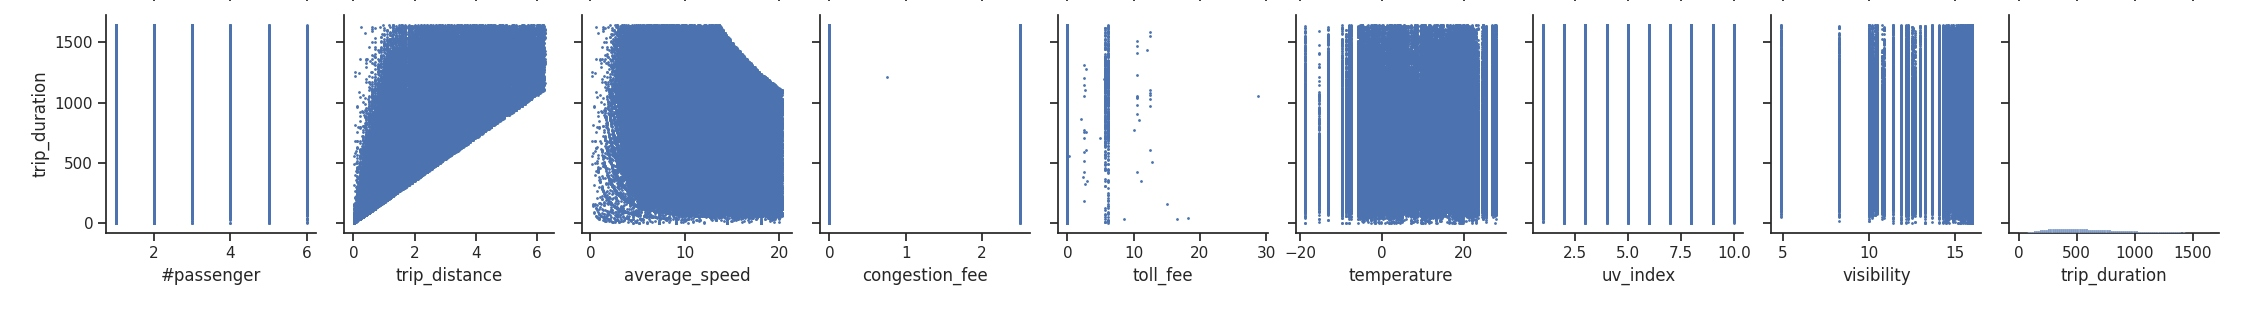
\includegraphics[width=1\textwidth]{part of pair plot.jpg}
  \caption{Part of Pair Plot for Continuous Features (sample size $=$ 0.01)}
  \vspace{-10pt}
  \label{fig:my_label}
\end{figure}

Next, we plotted Pearson and Spearman coefficient based heat maps for the continuous features. In the Pearson based heat map, \textit{trip distance} and \textit{trip duration} show a strong positive correlation, while \textit{average speed} shows a weak negative correlation. Meanwhile, the correlations of \textit{number of passengers} and \textit{visibility} are close to zero, and the other features show only weak positive correlation. In the Spearman-based heat map, although the overall correlation has increased, the overall trend has not changed significantly.

\begin{figure}[h!]
  \centering
  \begin{minipage}[b]{0.499\textwidth}
    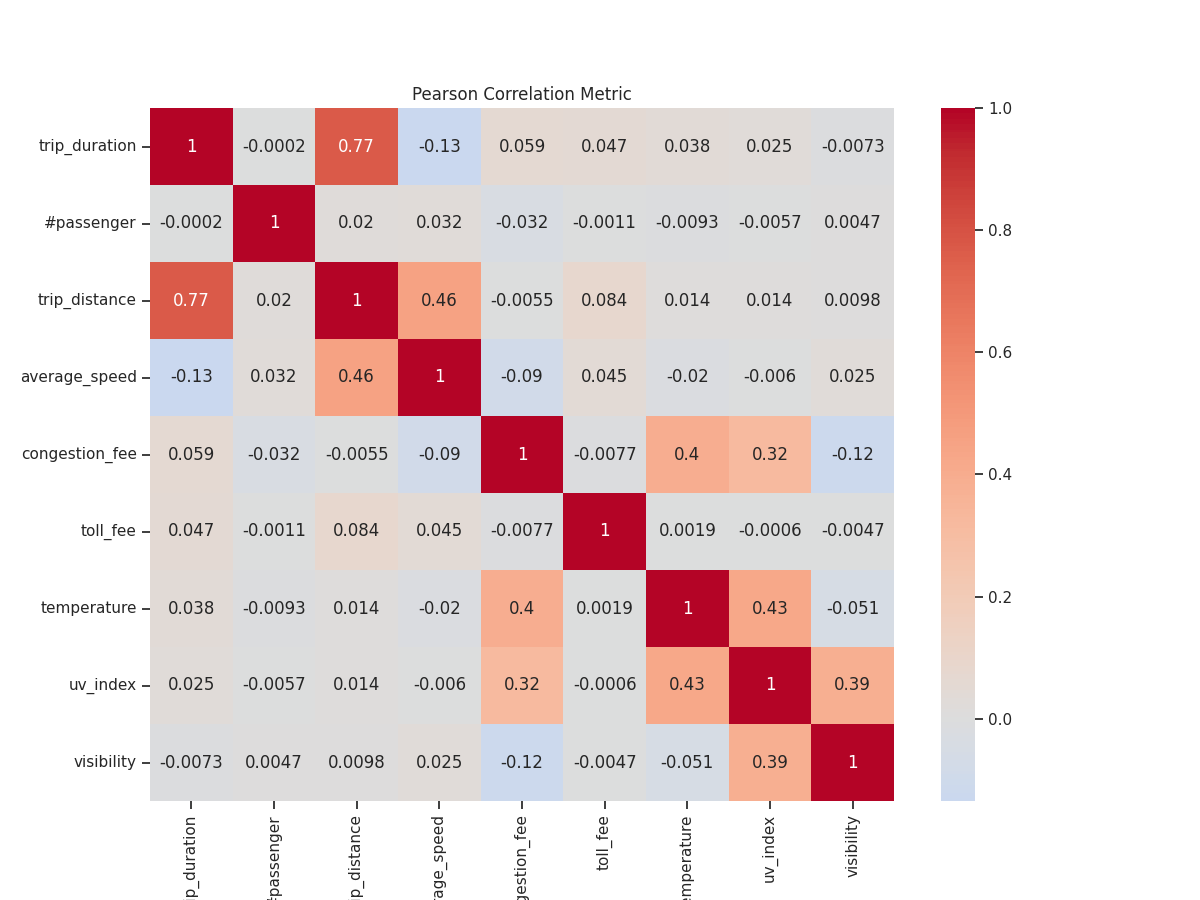
\includegraphics[width=\textwidth]{head_plot_for_continuous_features.png}
    \caption{Heat Plot for Continuous features (sample size $=$ 0.01)}
    %\vspace{1.05em}
    \label{fig:image1}
  \end{minipage}
  \hfill
  \begin{minipage}[b]{0.49\textwidth}
    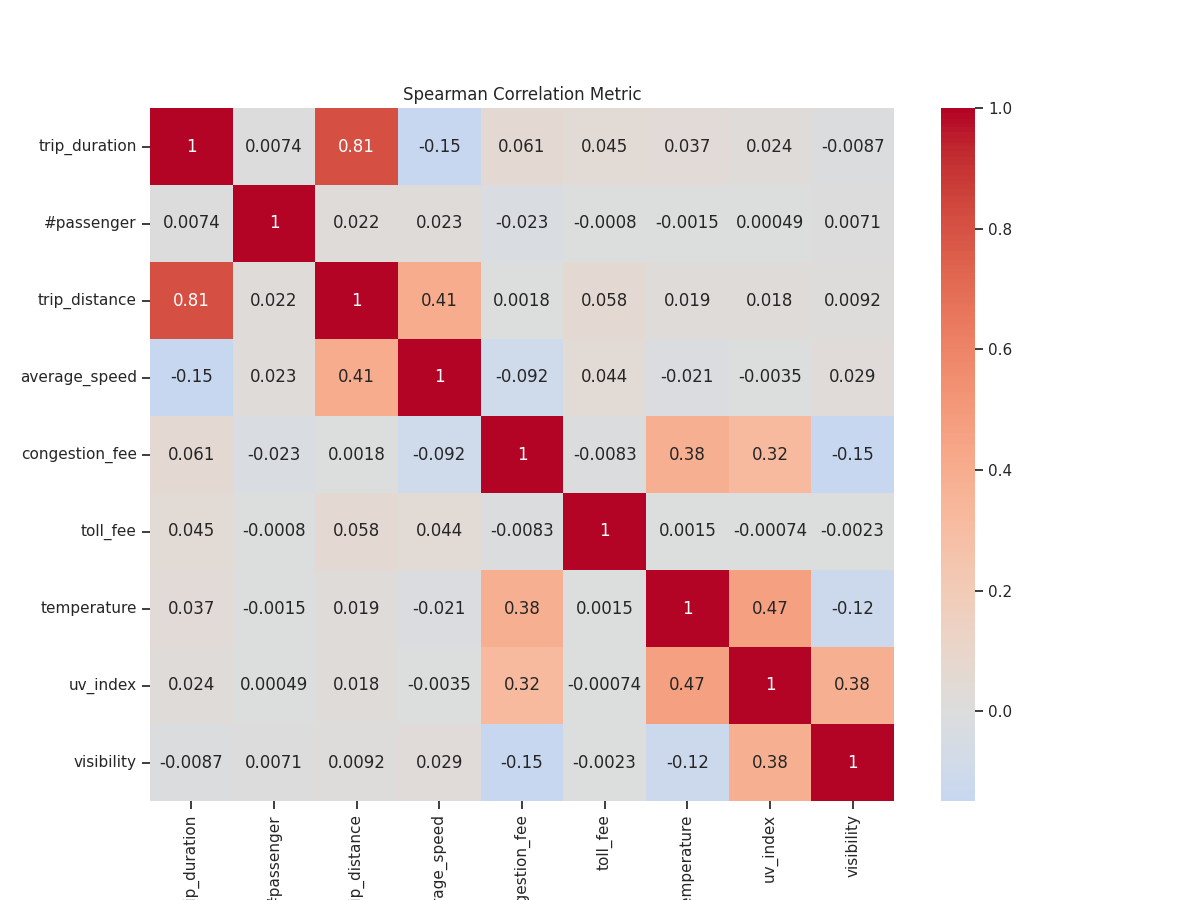
\includegraphics[width=\textwidth]{head_plot_with_spearman_for_continuous_features.png}
    \caption{Heat Plot with Spearman for Continuous features (sample size $=$ 0.01)}
    \label{fig:image2}
  \end{minipage}
\end{figure}

We further explored the correlation between \textit{trip duration} and the discrete features. Firstly, 1-way ANOVA was performed on the discrete features except for the 2 location features. The results showed that the $p$-values of these discrete features were all much less than 0.05, which means that they have a significant relationship with \textit{trip duration}(Table 2 (a)). Subsequently, we conducted a 2-way ANOVA with interaction for \textit{up\_location\_id} and \textit{off\_location\_id}. The results show that the $p$-values of both features and their interaction term are also much less than 0.05, indicating that they are significantly related to \textit{trip duration} not only have a significant relationship, but also an interaction effect(Table 2 (b)).

\begin{table}[h!]
    \centering

    \begin{minipage}{0.45\linewidth}
        \centering
        \subcaption{1-way ANOVA}
        \begin{tabular}{lr}
            \toprule
            Feature & p-value \\
            \midrule
            if\_overnight & 0.000000e+00 \\
            if\_peak\_hour & 1.283358e-128 \\
            if\_weekend & 2.001433e-62 \\
            if\_snow & 1.071452e-30 \\
            if\_airport & 1.947484e-17 \\
            if\_rain & 1.986263e-11 \\
            if\_clear & 1.102846e-03 \\
            if\_overcast & 2.390249e-03 \\
            if\_cloudy & 2.405049e-01 \\
            \bottomrule
        \end{tabular}
    \end{minipage}
    \hfill
    \begin{minipage}{0.45\linewidth}
        \centering
        \subcaption{2-way ANOVA with Interaction}
        \begin{tabular}{lr}
            \toprule
            Feature & p-value \\
            \midrule
            up\_location\_id & 1.500442e-21 \\
            off\_location\_id & 9.166038e-100 \\
            up\_location\_id:off\_location\_id & 1.065981e-286 \\
            Residual & NaN \\
            \bottomrule
        \end{tabular}
    \end{minipage}
    \caption{ANOVA for Discrete Features (sample size $=$ 0.01)}
\end{table}

\section{Modelling}

We selected the yellow taxi data of 2019.07 to be merged with the external data and then used as merged data for test. Merged data was sampled with the sample size of 0.004 to get the train set, while merged data for test was sampled with the sample size of 0.01 to get the test set. The inputs to the model have 6 continuous features and 12 discrete features: \textit{num of passengers}, \textit{trip\_distance}, \textit{congestion\_fee}, \textit{toll\_fee}, \textit{temperature}, \textit{uv\_index}, \textit{up\_location\_id}, \textit{off\_location\_id}, \textit{if\_weekend}, \textit{if\_peak\_hour}, \textit{if\_overnight}, \textit{if\_airport}, \textit{if\_rain}, \textit{if\_snow}, \textit{if\_overcast}, \textit{if\_cloudy}, \textit{if\_clear}, \textit{location\_interaction\_term}. The output of the model is \textit{trip\_duration}. \textit{date}, \textit{average\_speed}, \textit{visibility} were removed because the former was a feature used to merge the data, and the latter two had correlation coefficients close to 0 in the previous heatmap. \textit{location\_interaction\_term} was added because it proved to be significant in the previous anova test.

\subsection{Linear Regression Model}
The linear regression model learnt in machine learning is chosen because the prediction label is continuous variable. linear regression is highly interpretable, fast and suitable as a base line mode. The $R^2$ of the linear regression model is 0.6314 and 0.6041 on the train and test data, respectively, which means that the model explains more than 60\% of the variation in trip duration in the data and performs  consistently on the unknown data. The RMSE for the test data $RMSE = \sqrt(MSE) = \sqrt(49433.9984) = 222.34$ seconds, which is approximately 3.71 minutes. We believe that this error is acceptable for taxi trip duration prediction.


\subsection{Random Forest Regressor}
The random forest regressor is chosen because it can capture the nonlinear relationship between features and output and is robust to outliers\cite{scikit-learn_randomforest}\cite{sectionio_intro_randomforest}. The Random Forest regressor has an $R^2$ of 0.6953 and 0.6478 on the train and test sets, respectively, meaning that it explains about 5\% more variation than the linear regression model. The MSE of the Random Forest Regressor on the train and test sets is 37583.7094 and 43978.8330, respectively, which means that the Random Forest is more accurate on unknown data, with an error of about 209.71 seconds on the test set.

\section{Discussion}
\label{sec:discussion}
In Geospatial Visualisation section, we found that more than half of the 20 locations with the highest average trip durations are either sea-facing or islands. Upon closer inspection, we found that these locations were located far from the bridge. It is possible that these locations are a short straight line distance from their destination on a trip, but they need to go around the bridge that is far away. Therefore we reasonably suspect that the travelling needs of these locations are difficult to meet.

In Plotting and Analysis section, we find that all discrete features are significant for \textit{trip duration}, which contains 5 weather-related discrete features. We also found that \textit{pickup\_location} and \textit{dropoff\_location} have interactive effects on \textit{trip duration}.

In Modelling section, we think the features for predicting trip duration are generally efficient because the results of prediction are acceptable.

\section{Recommendations}
For the NYC department of transportation and roads: Travel demand on islands or coasts with high average trip duration could be met by building more bridges or providing more public transport such as ships.

For drivers and passengers who care about the trip duration: pay attention to the weather forecast, as weather conditions can and do affect the trip duration. However, temperature, UV intensity and visibility have a negligible effect on trip duration.

For yellow taxi companies looking to transition to online: focus on trip distance, weather, pick-up and drop-off locations and time of day as variables in predicting trip duration.


\section{Conclusion}
In general, in the data preprocessing step, we created new features for TLC data and external data, removed invalid or non-business rule rows and irrelevant or already extracted columns. Removed outliers for TLC data, and finally merged TLC data with the external data. In the analysis step, we plotted geopatial plots to see the \textit{average trip duration} for different locations. The distribution of "trip duration" was plotted. Then pair plot and heat map were plotted for continuous features and ANOVA was performed for discrete features to detect feature correlation. Finally, two models were developed to predict \textit{trip duration}.

\clearpage

% BEGIN REFERENCES SECTION
\printbibliography

\end{document}